\documentclass[a4paper,14pt]{extarticle}

\usepackage[top=1in, bottom=1in, left=1in, right=1in]{geometry}
\usepackage[utf8]{inputenc}
\usepackage[russian]{babel}
\usepackage[final]{graphicx}
\usepackage{caption}
\usepackage{subcaption}
\usepackage{chngcntr}
\usepackage{amsmath}
\usepackage{amsfonts}
\usepackage{pgfplots}
\usepackage{pgfplotstable}
\usepgfplotslibrary{fillbetween}
\usepackage{float}
\usepackage{lipsum}% http://ctan.org/pkg/lipsum
\usepackage{multicol}% http://ctan.org/pkg/multicol
\usepackage{hhline}
\usepackage{tabularx}
\usepackage{tikz,xcolor}
\usepackage{tkz-graph}
\usepackage{float}
\usepackage{mathtools}
\usepackage{todonotes}
\usepackage{listings}
\usepackage{epstopdf}
\usepackage{epsfig}
\usepackage[makeroom]{cancel}
\usepackage{subcaption}

\usetikzlibrary{arrows, petri, topaths}

\counterwithin{figure}{section}
\counterwithin{equation}{section}
\counterwithin{table}{section}

\DeclareMathOperator*{\argmin}{arg\,min}
\DeclareMathOperator*{\argmax}{arg\,max}
\DeclareMathOperator{\sinc}{sinc}

\definecolor{mygreen}{RGB}{28,172,0} % color values Red, Green, Blue
\definecolor{mylilas}{RGB}{170,55,241}

\lstset{language=Matlab,%
  %  basicstyle=\color{red},
    breaklines=true,%
    morekeywords={matlab2tikz,ylim,xlim,square,ones,double},
    keywordstyle=\color{blue},%
    morekeywords=[2]{1}, keywordstyle=[2]{\color{black}},
    identifierstyle=\color{black},%
    stringstyle=\color{mylilas},
    commentstyle=\color{mygreen},%
    showstringspaces=false,%without this there will be a symbol in the places where there is a space
    numbers=left,%
    numberstyle={ \color{black}},% size of the numbers
    numbersep=15pt, % this defines how far the numbers are from the text
    emph=[1]{for,end,break,switch,case,otherwise},emphstyle=[1]\color{red}, %some words to emphasise
    %emph=[2]{word1,word2}, emphstyle=[2]{style},    
}


\begin{document}
\begin{titlepage}
\centering 
{\bfseries Санкт-Петербургский Политехнический Университет} \\
Институт компьютерных наук и технологий \\
Кафедра компьютерных систем и программных технологий \\
\vspace{5cm}
{\centering \textbf{Отчёт по лабораторной работам №4 и №5} \\ 
\vspace{0.15cm}
\textbf{Дисциплина}: Телекоммуникационные технологии \\
\vspace{0.15cm}
\textbf{Тема}: Аналоговая модуляция. Фазовая и частотная модуляция.} \\
\vspace{4cm}
\hfill {\bfseries Работу выполнил студент}  \\
\hfill гр. 33501/4 Леженин Ю.И. \\
\hfill {\bfseries Преподаватель}  \\
\hfill Богач Н.В.
\vfill
Санкт-Петербург \\
{\large \today\par}
\end{titlepage}

\section{Цель работы.}

Изучение амплитудной модуляции/демодуляции сигнала. Изучение частотной и фазовой модуляции/демодуляции сигнала.

\section{Постановка задачи.} 

Сгенерировать однотональный сигнал низкой частоты. Выполнить амплитудную модуляцию/демодуляцию для различных значений глубины модуляции, амплитудную модуляцию/демодуляцию с подавлением несущей, однополосную модуляцию и синхронное детектирование. Выполнить фазовую и частотную модуляцию/демодуляцию. Получить спектры модулированных сигналов.


\section{Ход работы.}

\subsection{Амплитудная модуляция.}

Амплитудно-модулированный сигнал задается по закону
\begin{equation*}
u(t) = M \, U_m \, \cos(\Omega\,t) \, \cos(\omega_0 + \varphi_0),
\end{equation*}
где $M$ -- глубина модуляции, $\Omega$ -- частота модулируемого сигнала, $\omega_0$ -- несущая частота, а $\varphi_0$ -- начальная фаза. 

\begin{figure}[H]
\centering
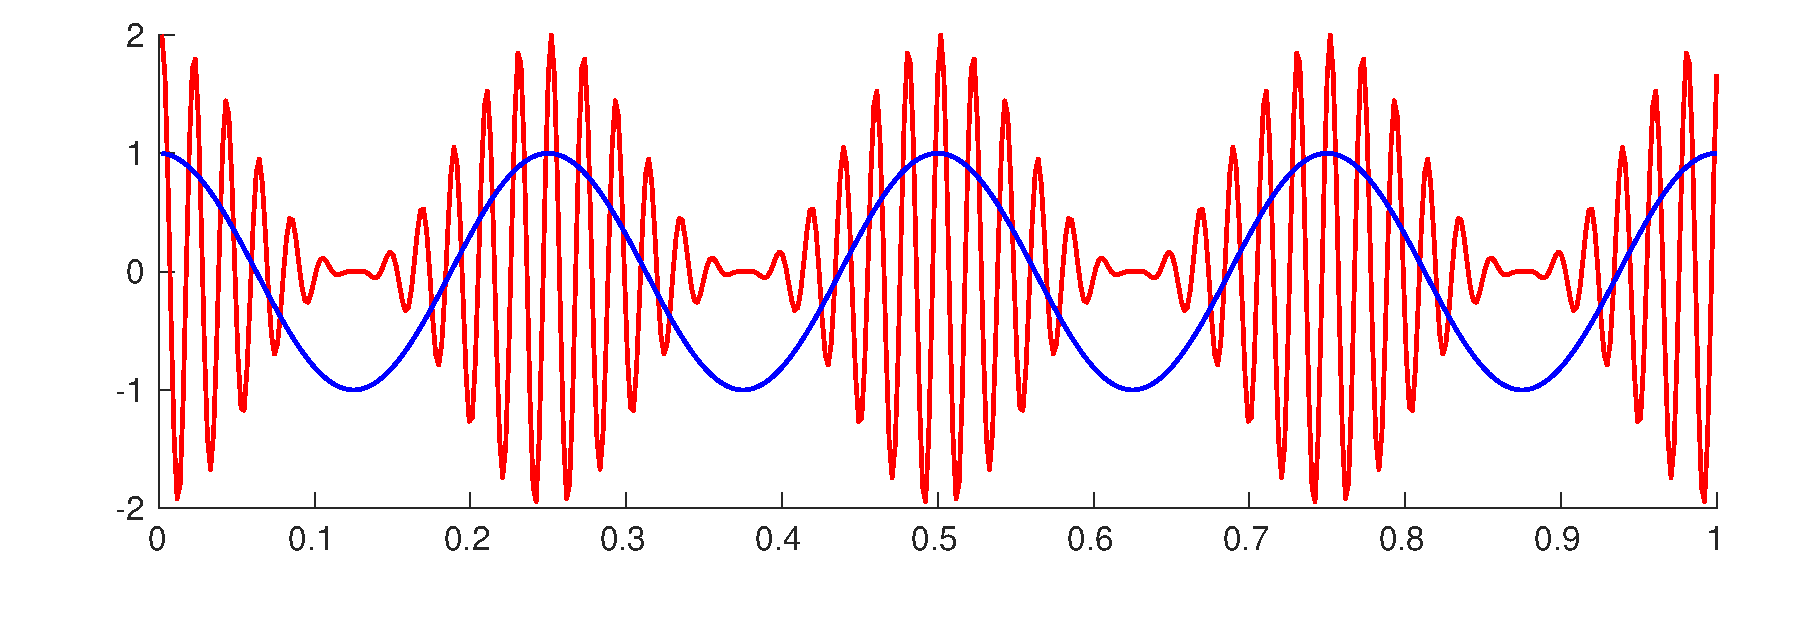
\includegraphics[width=0.95\textwidth]{ammod_m1.eps}
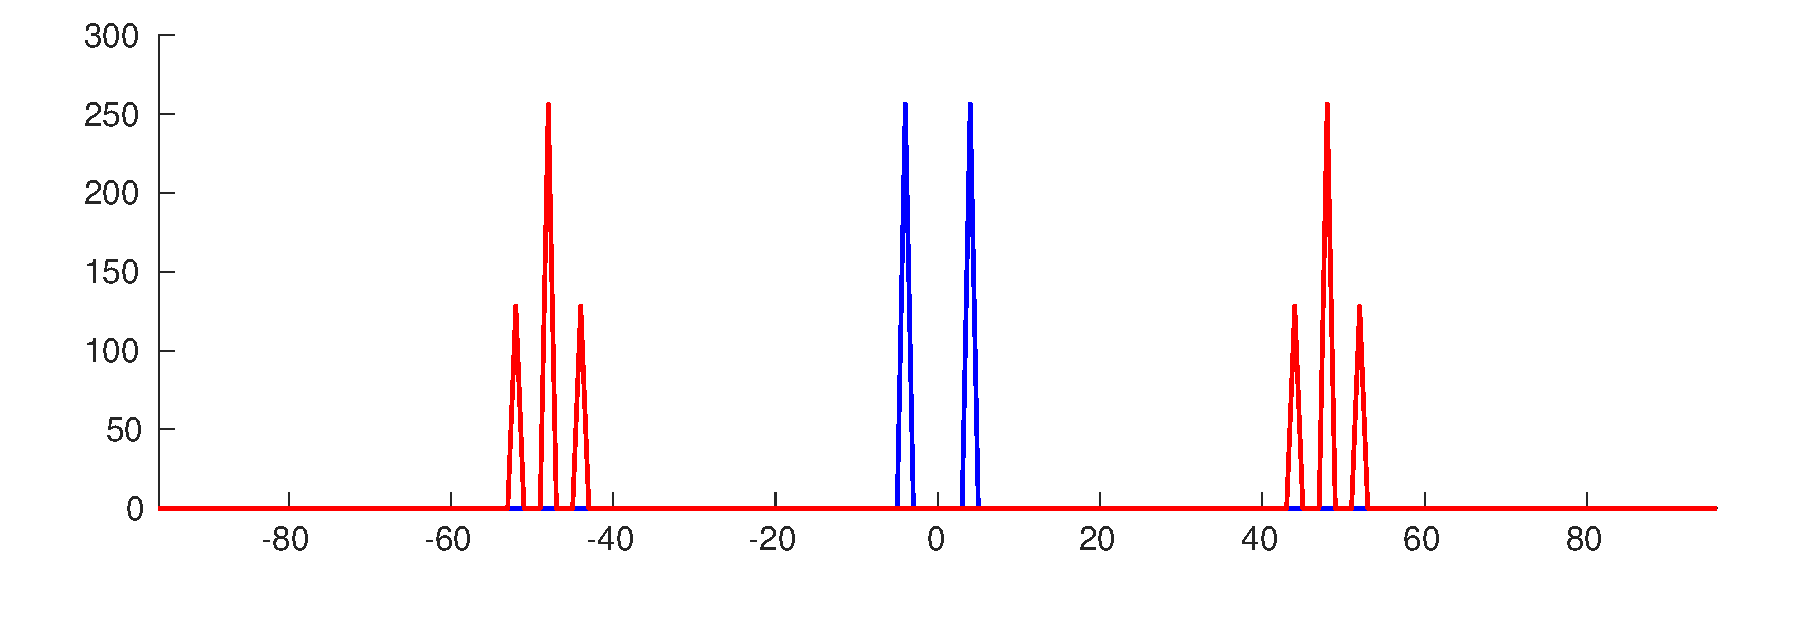
\includegraphics[width=0.95\textwidth]{ammod_s_m1.eps}
\captionsetup{justification=centering,margin=0.0cm}
\caption{Модулируемый однотональный сигнал ($\Omega = 4$ Гц), модулированный сигнал ($\omega_0 = 64$ Гц, $M = 1$) и их спектры.}
\label{sig}
\end{figure}

\begin{figure}[H]
\centering
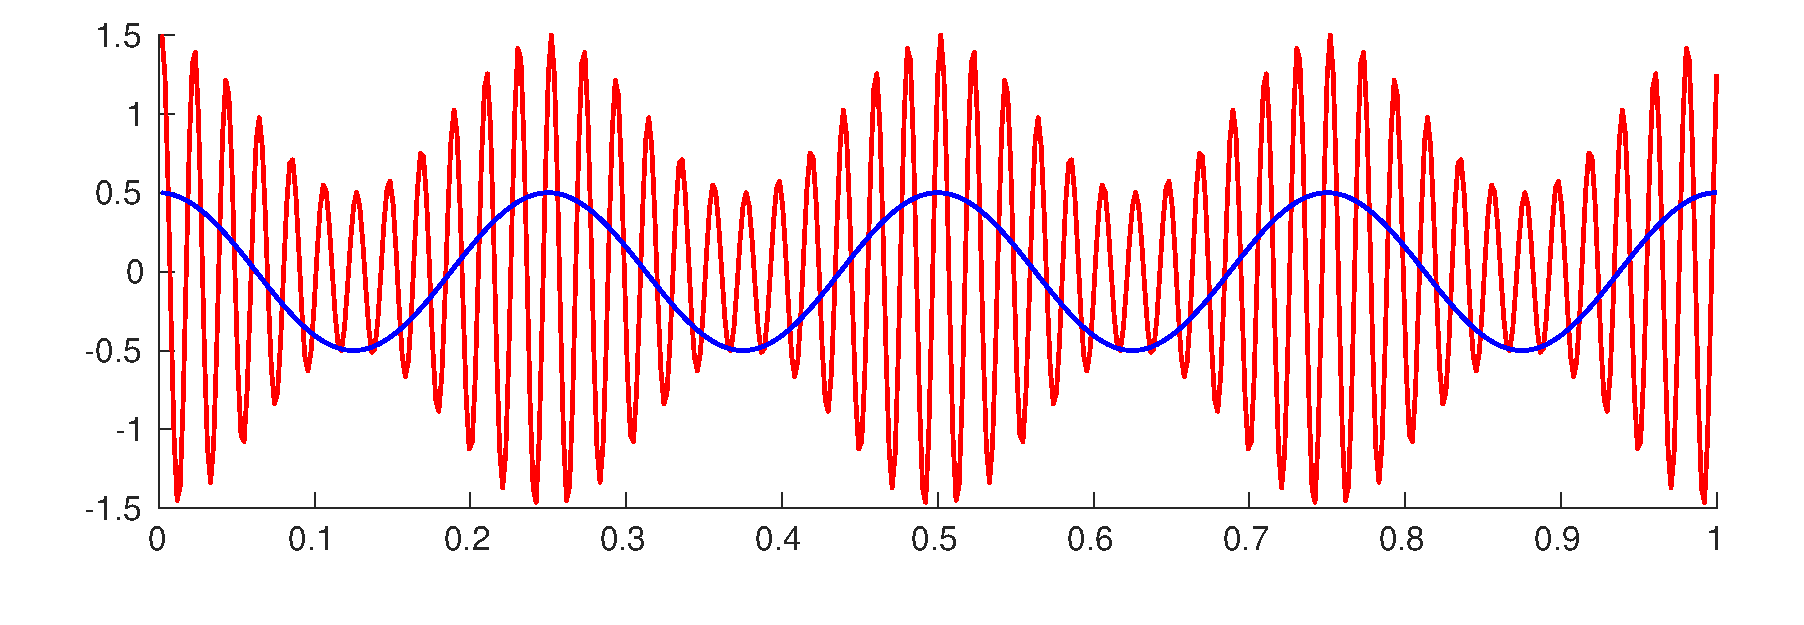
\includegraphics[width=0.95\textwidth]{ammod_m05.eps}
\includegraphics[width=0.95\textwidth]{ammod_s_m05.eps}
\captionsetup{justification=centering,margin=0cm}
\caption{Модулируемый однотональный сигнал ($\Omega = 4$ Гц), модулированный сигнал ($\omega_0 = 64$ Гц, $M = 0.5$) и их спектры.}
\label{sig}
\end{figure}

%\begin{figure}[H]
%\centering
%\includegraphics[width=\textwidth]{ammod_m1_s.eps}
%\captionsetup{justification=centering,margin=0.5cm}
%\caption{Спектр модулируемого однотонального сигнал с частотой $\Omega = 4$ Гц и амплитудно-модулированный сигнал с несущей частотой $\omega_0 = 64$ Гц и глубиной модуляции $m = 1$. }
%\label{sig}
%\end{figure}

\section{Выводы.}

Линейный цепи позволяют осуществлять фильтрацию сигнала, т.е. целенаправленным образом менять спектр сигнала. Это позволяет повысить отношение полезного сигнала к шумам и помехам.

По виду амплитудно-частотной характеристики фильтры делятся на 4 типа: ФНЧ, ФВЧ, ФПП, ФПЗ.
По виду импульсной характеристики выделяют КИХ-фильтры и БИХ-фильтры.



\section{Приложение.}

\lstinputlisting[frame=single, caption=Программа для выполнения амплитудной модуляции/демодуляции.]{lab4_script.m}


\end{document}